% This file was created by tikzplotlib v0.9.1.
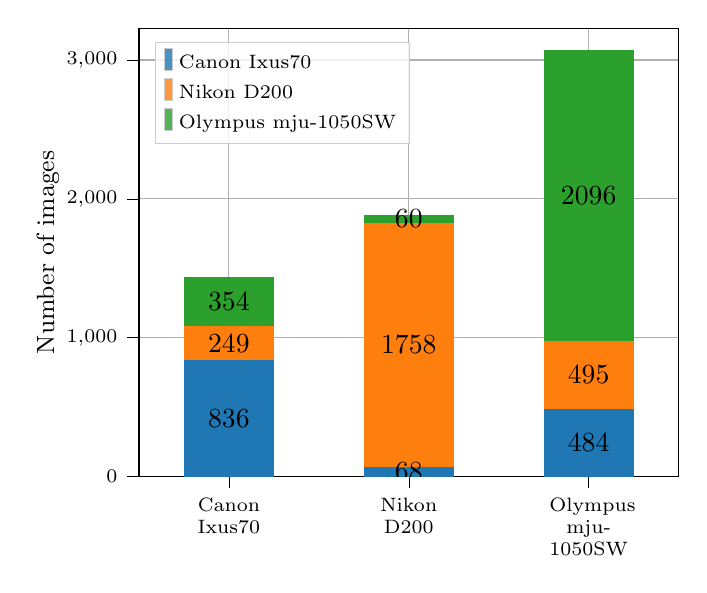
\begin{tikzpicture}

\definecolor{color0}{rgb}{0.12156862745098,0.466666666666667,0.705882352941177}
\definecolor{color1}{rgb}{1,0.498039215686275,0.0549019607843137}
\definecolor{color2}{rgb}{0.172549019607843,0.627450980392157,0.172549019607843}

\pgfplotsset{compat=1.11,
	/pgfplots/ybar legend/.style={
		/pgfplots/legend image code/.code={%
			\draw[##1,/tikz/.cd,yshift=-0.25em]
			(0cm,0cm) rectangle (3pt,0.8em);},
	}, every tick label/.append style={font=\scriptsize}
}

\begin{axis}[
legend cell align={left},
legend style={fill opacity=0.8, draw opacity=1, text opacity=1, at={(0.03,0.97)}, anchor=north west, draw=white!80!black},
tick align=outside,
tick pos=left,
grid=major,
x grid style={white!69.0196078431373!black},
xmin=-0.5, xmax=2.5,
xtick style={color=black},
xtick={0,1,2},
xticklabel style={text width=1cm, align=center},
xticklabels={Canon Ixus70,Nikon D200,Olympus mju-1050SW},
y grid style={white!69.0196078431373!black},
ymin=0, ymax=3228.75,
ytick style={color=black},
y label style={at={(axis description cs:-0.13,.5)},anchor=south},
ylabel={\small Number of images}
]
\draw[draw=none,fill=color0] (axis cs:-0.25,0) rectangle (axis cs:0.25,836);
\addlegendimage{ybar,ybar legend,draw=none,fill=color0};
\addlegendentry{\scriptsize Canon Ixus70}

\draw[draw=none,fill=color0] (axis cs:0.75,0) rectangle (axis cs:1.25,68);
\draw[draw=none,fill=color0] (axis cs:1.75,0) rectangle (axis cs:2.25,484);
\draw[draw=none,fill=color1] (axis cs:-0.25,836) rectangle (axis cs:0.25,1085);
\addlegendimage{ybar,ybar legend,draw=none,fill=color1};
\addlegendentry{\scriptsize Nikon D200}

\draw[draw=none,fill=color1] (axis cs:0.75,68) rectangle (axis cs:1.25,1826);
\draw[draw=none,fill=color1] (axis cs:1.75,484) rectangle (axis cs:2.25,979);
\draw[draw=none,fill=color2] (axis cs:-0.25,1085) rectangle (axis cs:0.25,1439);
\addlegendimage{ybar,ybar legend,draw=none,fill=color2};
\addlegendentry{\scriptsize Olympus mju-1050SW}

\draw[draw=none,fill=color2] (axis cs:0.75,1826) rectangle (axis cs:1.25,1886);
\draw[draw=none,fill=color2] (axis cs:1.75,979) rectangle (axis cs:2.25,3075);
\draw (axis cs:0,418) node[
  scale=1,
  text=black,
  rotate=0.0
]{836};
\draw (axis cs:1,34) node[
  scale=1,
  text=black,
  rotate=0.0
]{68};
\draw (axis cs:2,242) node[
  scale=1,
  text=black,
  rotate=0.0
]{484};
\draw (axis cs:0,960.5) node[
  scale=1,
  text=black,
  rotate=0.0
]{249};
\draw (axis cs:1,947) node[
  scale=1,
  text=black,
  rotate=0.0
]{1758};
\draw (axis cs:2,731.5) node[
  scale=1,
  text=black,
  rotate=0.0
]{495};
\draw (axis cs:0,1262) node[
  scale=1,
  text=black,
  rotate=0.0
]{354};
\draw (axis cs:1,1856) node[
  scale=1,
  text=black,
  rotate=0.0
]{60};
\draw (axis cs:2,2027) node[
  scale=1,
  text=black,
  rotate=0.0
]{2096};
\end{axis}

\end{tikzpicture}
